\chapter{Getting started}
\newpage
\section{Welcome}
This is the manual for Rockbox.  Rockbox is a replacement firmware for the
Jukebox Studio, Recorder and Ondio players made by Archos, the H120/140
players from iRiver and the Apple iPod Nano etc.  It is a complete rewrite of
the software used to make the PDA play and record music, and contains many
features and enhancements not available in the original firmware supplied by
the manufacturer.  Among the things that Rockbox has to offer are the
following:

\begin{itemize}
\item Faster loading than the \playername firmware
\item Uninterrupted playing of MP3 files {--} skipping is very rare
\item More control over how your music is played
\item Built in viewers for several common file types
\item Sophisticated plugin system that allows the Jukebox to run games,
a calendar, a clock, and many other applications.
\item Totally removable. (Removal of Rockbox before returning the
Jukebox for repair under warranty is advised.)
\item Optional voice user interface for complete control without looking
at the screen
\end{itemize}
Rockbox is a complete from scratch rewrite of the \playername software and
uses no fragments of the original firmware.  Not only is it free to
use, it's also released under the GNU public license,
which means that it will always remain free to both use and to change.

\opt{OndioSP,OndioFM}{Although Rockbox also runs on the Archos Ondio series of
flash based MP3 players,  this is a recent development, which is not covered
fully in this manual.  Most of this manual will, however, apply equally to
Rockbox on the Ondio Jukeboxes.  For more details on the Ondio port, please
see the web page:
\url{http://www.rockbox.org/twiki/bin/view/Main/ArchosOndio}.}

\section{Getting more help}

This manual is intended to be a comprehensive introduction to the Rockbox
software.  There is, however, more help available.  The Rockbox website at
\url{http://www.rockbox.org/}contains very extensive documentation and guides
written by members of the Rockbox community and this should be your first port
of call when looking for further help.

\opt{Archos}{\section{Before installation}

Before you install Rockbox, you will need to know what model you own.  Rockbox 
comes in different versions depending on the model of your \dap{}.  There are 
six different versions of the software.  The table below will help you to 
identify which version of the software you need.

The model name is printed on the case.  The hard drive size is listed on the
serial number sticker on the back of the unit.

\begin{center}
  \begin{tabularx}{\textwidth}{llXl}\toprule
    \label{ref:Jukeboxtypetable}
    \textbf{Picture} & \textbf{Disk size} & \textbf{Model Name} & \textbf{Version Name} \\\midrule
    \begin{minipage}{2.2cm}
      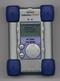
\includegraphics[width=2cm]{getting_started/images/archos-studio-small.png}
    \end{minipage} 
    & 5GB, 6GB, 10GB, 20GB & 
                             \begin{minipage}{8cm}
                             Jukebox 5000 \newline
                             Jukebox 6000 \newline
                             Jukebox Studio 10 \newline
                             Jukebox Studio 20
                             \end{minipage}
                               & player \\\midrule
    \begin{minipage}{2.2cm}
      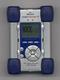
\includegraphics[width=2cm]{getting_started/images/archos-recorder-small.png}
    \end{minipage}
    & 6GB, 10GB, 15GB, 20GB & \begin{minipage}{8cm}
                              Jukebox Recorder 6 \newline
                              Jukebox Recorder 10 \newline
                              Jukebox Recorder 15 \newline
                              Jukebox Recorder 20 
                              \end{minipage}
                               & recorder\\\midrule
    \begin{minipage}{2.2cm}
      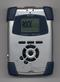
\includegraphics[width=2cm]{getting_started/images/archos-recorderv2-small.png}
    \end{minipage}
                     & 20GB & Jukebox Recorder v2 & recorderv2\\\midrule
    \begin{minipage}{2.2cm}
      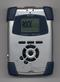
\includegraphics[width=2cm]{getting_started/images/archos-recorderfm-small.png}
    \end{minipage}
                     & 20GB & Jukebox Recorder FM & fmrecorder \\\midrule
    \begin{minipage}{2.2cm}
      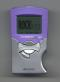
\includegraphics[width=2cm]{getting_started/images/archos-ondiosp-small.png}
    \end{minipage}
                     & 128MB (flash) & Ondio 128 SP & ondiosp \\\midrule
    \begin{minipage}{2.2cm}
      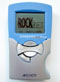
\includegraphics[width=2cm]{getting_started/images/archos-ondiofm-small.png}
    \end{minipage}
                     & 128MB (flash) & Ondio 128 FM & ondiofm \\\bottomrule
  \end{tabularx}
\end{center}
\note{Rockbox does not run on the Archos Jukebox Multimedia or any
Archos products other than those mentioned here.}
}


\section{Downloading Rockbox}

The latest release of the Rockbox software will always be available from
\url{http://www.rockbox.org/download/}.
 Windows users may wish to download the self{}-extracting Windows
installer, which works for all Jukebox models, but those wishing to
install manually or using a different operating system should choose
the .zip archive containing the firmware for their model of the
Jukebox.

\section{Installing Rockbox}

Using the Windows self installing executable to install Rockbox is the easiest
method of installing the software on your Jukebox.  Simply follow the
on{}-screen instructions and select the appropriate drive letter and Jukebox
model when prompted.  You can use ``Add / Remove Programs'' to uninstall the
software at a later date.

For non{}-Windows users and those wishing to install manually from the archive
the procedure is still fairly simple.  Connect your \playername to the computer
via USB as described in the manual that came with your \playername. On Windows,
the \playername drive will appear as a drive letter in your ``My Computer''
folder. Take the file that you downloaded above, and unpack its contents to
your \playername drive. You can do this using a program such as
\url{http://www.info-zip.org/} or \url{http://www.winzip.org/}. 

You will need to unpack all of the files in the archive onto your hard
disk. If this has been done correctly, you will have a file called
\opt{PS}{\fname{archos.mod}}
\opt{Rec,Rec2,FMRec}{\fname{ajbrec.ajz}}
\opt{H120,H340}{\fname{rockbox.iriver}}
in the main folder of your \playername drive, and also a folder called
/\fname{.rockbox}, which contains a number of system files used by the
software.

\section{Enabling Speech Support (optional)}

If you wish to use speech support you will also need a language file,
available from
\url{http://www.rockbox.org/twiki/bin/view/Main/VoiceFiles/}.
 For the English language, the file is called \fname{english.voice}.
When it has been downloaded, unpack this file and copy it into the
\fname{lang} folder which is inside the /\fname{.rockbox} folder on
your Jukebox. Voice menus are turned on by default.  See page
\pageref{ref:Voiceconfiguration} for details on voice settings.


\section{Running Rockbox}

Remove your Jukebox from the computer's USB port.
Unplug any connected power supply and turn the unit off. When you next
turn the unit on, the Jukebox firmware will start to load, and then it
will load Rockbox for you. When you see the Rockbox splash screen,
Rockbox is loaded and ready for use. 

\section{Uninstalling Rockbox}

If you would like to go back to using the
original \playername software, then connect the \playername up to your computer,
and delete the 
\opt{PS}{\fname{archos.mod}}
\opt{Rec,Rec2,FMRec}{\fname{ajbrec.ajz}}
\opt{H120,H340}{\fname{rockbox.iriver}}
If you wish to clean up your disk, you may also wish to delete the
\fname{.rockbox} folder and its contents. Turn the \playername off and on and
the normal \playername software will load.
